\section{Analisi del Dominio}
\frame{\tableofcontents[currentsection]}

%-------------------------------------------------
\subsection{Analisi del Problema}

\begin{frame}
    \frametitle{Analisi del Problema}
    È stata condotta un'intervista con degli esperti di dominio che hanno consentito di chiarire quale sia l'attuale
    funzionamento del sistema.
    Questi hanno inoltre espresso i miglioramenti che desiderano vengano introdotti nella gestione della raccolta dei
    rifiuti.

    \bigskip

    Grazie alle risposte ottenute è stato possibile costruire un \textbf{Ubiquitous Language} condiviso tra il team di sviluppo
    e l'azienda.

\end{frame}
%------------------------------------------------

%-------------------------------------------------
\subsection{Ubiquitous Language}

\begin{frame}
    \frametitle{Ubiquitous Language}
    Grazie all'appronfondita analisi del dominio che è stata effettuata con i committenti, il team ha prodotto un
    \textbf{Ubiquitous Language}.

    \bigskip

    La costruzione di questo vocabolario ha consentito a tutti i membri del team di avere chiaro quali siano gli
    elementi che sono presenti all'interno del dominio e quali siano i loro ruoli, rimuovendo tutte le ambiguità.

    \bigskip

    L'Ubiquitous Language ha consentito agli sviluppatori di lavorare in modo indipendente e parallelo su componenti
    differenti del sistema.

\end{frame}
%------------------------------------------------

%-------------------------------------------------
\subsection{Analisi dell'Impatto}

\begin{frame}
    \frametitle{Analisi dell'Impatto}
    Per fare chiarezza con l'organizzazione sull'impatto del progetto è stato realizzato un \textbf{Impact Mapping}.

    \smallskip

    \begin{figure}[H]
        \centering
        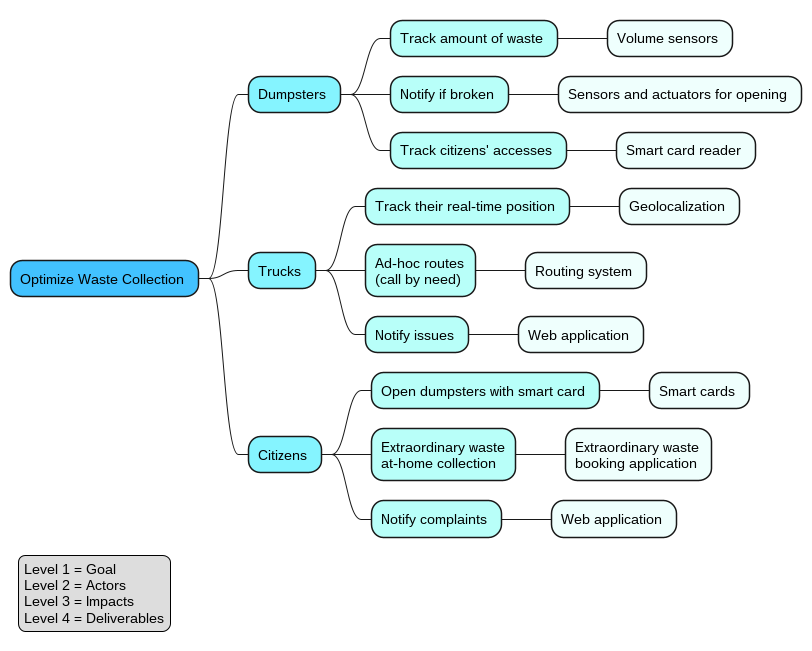
\includegraphics[width=0.7\linewidth]{../img/impact-mapping}
    \end{figure}

\end{frame}
%------------------------------------------------
